\documentclass[12pt,a4paper]{article}
\usepackage[utf8]{vietnam}
\usepackage{amsmath,amssymb,amsfonts,mathrsfs}
\usepackage[left=1.5cm,right=1.5cm,top=2cm,bottom=2cm,headheight=17pt]{geometry}
\usepackage{enumitem}
\usepackage{array}
\usepackage{graphicx}
\usepackage{tikz}
\usetikzlibrary{arrows.meta,calc,patterns}
\usepackage{fancyhdr}

\pagestyle{fancy}
\fancyhf{}
\lhead{\small\textbf{HƯỚNG TỚI THPTQG 2027}}
\rhead{\small\textit{Người biên soạn: Dương Gia Bảo}}
\rfoot{\small Trang \thepage}
\renewcommand{\headrulewidth}{0.4pt}

\begin{document}

\noindent
\begin{minipage}[t]{0.40\textwidth}
    \centering
    \textbf{HƯỚNG TỚI THPTQG 2027}\\[-2pt]
    \rule{3.2cm}{0.6pt}\\[4pt]
    \textbf{ĐỀ CHÍNH THỨC}
\end{minipage}\hfill
\begin{minipage}[t]{0.58\textwidth}
    \centering
    \textbf{ĐỀ THI KHẢO SÁT CHẤT LƯỢNG}\\
    \textbf{ĐỀ SỐ 10}\\
    \textbf{Môn thi: TOÁN}\\
    \textit{\small Thời gian làm bài: 90 phút, không kể thời gian phát đề}
\end{minipage}

\vspace{0.2cm}
\noindent
\begin{minipage}[b]{0.78\textwidth}
    \textbf{Họ và tên:}\dotfill\textbf{SBD:}\makebox[3.5cm]{\dotfill}
\end{minipage}\hfill
\begin{minipage}[b]{0.20\textwidth}
    \hfill
    \setlength{\fboxrule}{0.8pt}%
    \fbox{\begin{minipage}{2.3cm}
        \centering
        \textbf{\small Mã đề thi}\\
        \textbf{0010}
    \end{minipage}}
\end{minipage}
\vspace{0.2cm}

% ==========================================
% PHẦN I
% ==========================================
\section*{\large PHẦN I. CÂU TRẮC NGHIỆM NHIỀU PHƯƠNG ÁN LỰA CHỌN}
\textit{Thí sinh trả lời từ câu 1 đến câu 12. Mỗi câu hỏi thí sinh chỉ chọn một phương án. Mỗi câu trả lời đúng được 0,25 điểm.}

\begin{enumerate}[label=\textbf{Câu \arabic*:}, leftmargin=*]

\item Cho hàm số $y = \dfrac{2x^2 + x - 3}{x + 1}$ có đồ thị $(C)$. Đường tiệm cận xiên của đồ thị $(C)$ có phương trình là
\begin{enumerate}[label=\Alph*.]
    \item $y = 2x + 1$.
    \item $y = 2x - 1$.
    \item $y = x - 1$.
    \item $y = 2x - 3$.
\end{enumerate}

\item Tập xác định $D$ của hàm số $y = \dfrac{\ln(9 - x^2)}{x - 1}$ là
\begin{enumerate}[label=\Alph*.]
    \item $D = (-3; 3)$.
    \item $D = [-3; 3] \setminus \{1\}$.
    \item $D = (1; 3)$.
    \item $D = (-3; 3) \setminus \{1\}$.
\end{enumerate}

\item Họ tất cả các nguyên hàm của hàm số $f(x) = \dfrac{1}{2x + 3}$ trên khoảng $\left(-\dfrac{3}{2}; +\infty\right)$ là
\begin{enumerate}[label=\Alph*.]
    \item $F(x) = \dfrac{1}{2}\ln(2x + 3) + C$.
    \item $F(x) = \ln(2x + 3) + C$.
    \item $F(x) = 2\ln(2x + 3) + C$.
    \item $F(x) = -\dfrac{1}{2}\ln(2x + 3) + C$.
\end{enumerate}

\item Trong không gian $Oxyz$, cho đường thẳng $d: \dfrac{x - 1}{2} = \dfrac{y + 3}{-3} = \dfrac{z - 5}{5}$. Vectơ nào dưới đây là một vectơ chỉ phương của đường thẳng $d$?
\begin{enumerate}[label=\Alph*.]
    \item $\vec{u}_1 = (2; 3; 5)$.
    \item $\vec{u}_2 = (1; -3; 5)$.
    \item $\vec{u}_3 = (-4; 6; -10)$.
    \item $\vec{u}_4 = (-2; -3; 5)$.
\end{enumerate}

\item Một hệ thống cảnh báo an ninh gồm hai cảm biến hoạt động độc lập với nhau. Xác suất để cảm biến thứ nhất kích hoạt báo động khi xảy ra sự cố là $0{,}8$; xác suất để cảm biến thứ hai kích hoạt khi xảy ra sự cố là $0{,}7$. Khi có sự cố xảy ra, xác suất để có ít nhất một trong hai cảm biến kích hoạt báo động thành công bằng
\begin{enumerate}[label=\Alph*.]
    \item $0{,}56$.
    \item $0{,}94$.
    \item $0{,}86$.
    \item $0{,}90$.
\end{enumerate}

\item Thời gian hoàn thành một công đoạn lắp ráp sản phẩm (đơn vị: phút) của $40$ công nhân tại một nhà xưởng được ghi nhận trong bảng số liệu ghép nhóm sau:
\begin{center}
\begin{tabular}{|c|c|c|c|c|c|}
\hline
\textbf{Thời gian (phút)} & $[4; 5)$ & $[5; 6)$ & $[6; 7)$ & $[7; 8)$ & $[8; 9)$ \\ \hline
\textbf{Số công nhân} & 4 & 8 & 14 & 10 & 4 \\ \hline
\end{tabular}
\end{center}
Tứ phân vị thứ nhất $Q_1$ của mẫu số liệu ghép nhóm trên bằng
\begin{enumerate}[label=\Alph*.]
    \item $5{,}50$.
    \item $5{,}60$.
    \item $6{,}25$.
    \item $5{,}75$.
\end{enumerate}

\item Cho hình chóp $S.ABC$ có đáy $ABC$ là tam giác vuông tại $B$, $AB = a$, $BC = a\sqrt{2}$. Cạnh bên $SA$ vuông góc với mặt phẳng đáy và $SA = a$. Số đo của góc nhị diện $[S, BC, A]$ bằng
\begin{enumerate}[label=\Alph*.]
    \item $45^\circ$.
    \item $60^\circ$.
    \item $30^\circ$.
    \item $90^\circ$.
\end{enumerate}

\item Cho cấp số nhân $(u_n)$ có số hạng đầu $u_1 = 2$ và công bội $q = -3$. Số hạng thứ tư $u_4$ của cấp số nhân bằng
\begin{enumerate}[label=\Alph*.]
    \item $54$.
    \item $-162$.
    \item $-54$.
    \item $18$.
\end{enumerate}

\item Độ pH của một dung dịch được xác định bởi công thức $\text{pH} = -\log_{10}[H^+]$, trong đó $[H^+]$ là nồng độ ion hydrogen tính theo $\text{mol/L}$. Một mẫu dung dịch ban đầu có nồng độ $[H^+] = 10^{-5}\text{ mol/L}$. Sau khi pha thêm nước tinh khiết, nồng độ ion hydrogen giảm xuống còn $[H^+] = 10^{-7}\text{ mol/L}$. Khi đó độ pH của dung dịch thay đổi như thế nào?
\begin{enumerate}[label=\Alph*.]
    \item Giảm đi 2 đơn vị.
    \item Tăng thêm 2 đơn vị.
    \item Tăng thêm 100 đơn vị.
    \item Giảm đi 100 đơn vị.
\end{enumerate}

\item Trong không gian $Oxyz$, cho mặt cầu $(S): x^2 + y^2 + z^2 - 4x + 2y - 6z + 5 = 0$. Tọa độ tâm $I$ và bán kính $R$ của mặt cầu $(S)$ là
\begin{enumerate}[label=\Alph*.]
    \item $I(-2; 1; -3), R = 3$.
    \item $I(2; -1; 3), R = 9$.
    \item $I(-4; 2; -6), R = 3$.
    \item $I(2; -1; 3), R = 3$.
\end{enumerate}

\item Một xưởng thủ công mỹ nghệ ước tính chi phí để sản xuất $x$ sản phẩm ($0 \le x \le 100$) là $C(x) = 20x + 100$ (nghìn đồng) và doanh thu thu về tương ứng là $R(x) = 120x - x^2$ (nghìn đồng). Để xưởng thu được lợi nhuận lớn nhất thì cần sản xuất bao nhiêu sản phẩm?
\begin{enumerate}[label=\Alph*.]
    \item $50$.
    \item $60$.
    \item $40$.
    \item $70$.
\end{enumerate}

\item Cho hình lăng trụ đứng $ABC.A'B'C'$ có đáy $ABC$ là tam giác vuông tại $A$ với $AB = 3a, AC = 4a$. Biết thể tích của khối lăng trụ bằng $36a^3$. Độ dài cạnh bên $AA'$ bằng
\begin{enumerate}[label=\Alph*.]
    \item $3a$.
    \item $4a$.
    \item $6a$.
    \item $12a$.
\end{enumerate}

\end{enumerate}

% ==========================================
% PHẦN II
% ==========================================
\vspace{0.4cm}
\section*{\large PHẦN II. CÂU TRẮC NGHIỆM ĐÚNG SAI}
\textit{Thí sinh trả lời từ câu 1 đến câu 4. Trong mỗi ý \textbf{a)}, \textbf{b)}, \textbf{c)}, \textbf{d)} ở mỗi câu, thí sinh chọn đúng hoặc sai.}

\begin{enumerate}[label=\textbf{Câu \arabic*:}, leftmargin=*]

\item Cho hàm số $y = \dfrac{x^2 - x + 1}{x - 1}$ có đồ thị $(C)$.
\begin{enumerate}[label=\textbf{\alph*)}]
    \item Hàm số đạt cực đại tại $x = 0$ và đạt cực tiểu tại $x = 2$.
    \item Đường thẳng đi qua hai điểm cực trị của đồ thị $(C)$ có phương trình $y = 2x - 1$.
    \item Giao điểm của hai đường tiệm cận của đồ thị $(C)$ là điểm $I(1; 2)$.
    \item Tiếp tuyến của đồ thị $(C)$ tại điểm có hoành độ $x = 2$ song song với trục hoành $Ox$.
\end{enumerate}

\item Trong một chương trình tầm soát một căn bệnh di truyền hiếm gặp ở một cộng đồng dân cư, tỉ lệ người thực sự mắc bệnh là $1\%$. Một phương pháp xét nghiệm chẩn đoán y tế có độ nhạy là $98\%$ (xác suất người có bệnh nhận kết quả dương tính) và độ đặc hiệu là $95\%$ (xác suất người không có bệnh nhận kết quả âm tính). Chọn ngẫu nhiên một người trong cộng đồng để thực hiện xét nghiệm.
\begin{enumerate}[label=\textbf{\alph*)}]
    \item Xác suất để một người được chọn ngẫu nhiên có kết quả xét nghiệm dương tính bằng $0{,}0593$.
    \item Nếu một người có kết quả xét nghiệm dương tính thì xác suất người đó thực sự mắc bệnh lớn hơn $50\%$.
    \item Xác suất để một người được chọn ngẫu nhiên vừa không mắc bệnh vừa nhận kết quả xét nghiệm âm tính bằng $0{,}9405$.
    \item Nếu một người nhận kết quả xét nghiệm âm tính thì xác suất người đó vẫn mắc bệnh nhỏ hơn $0{,}05\%$.
\end{enumerate}

\item \begin{minipage}[t]{0.55\linewidth}
Một trạm kiểm soát không lưu đặt thiết bị radar cảnh giới tại gốc tọa độ $O(0; 0; 0)$ trong không gian $Oxyz$ (đơn vị đo trên các trục là ki-lô-mét). Tại thời điểm $t = 0$ (giờ), một thiết bị bay không người lái (drone) xuất phát từ điểm $A(8; 6; 4)$ và di chuyển theo đường thẳng với vận tốc không đổi được mô tả bởi vectơ $\vec{v} = (-2; -1; 1)$ (km/h). Vị trí của drone tại thời điểm $t$ ($t \ge 0$) là điểm $M(8 - 2t; 6 - t; 4 + t)$.
\begin{enumerate}[label=\textbf{\alph*)}]
    \item Khoảng cách từ trạm radar $O$ đến vị trí xuất phát $A$ của drone bằng $2\sqrt{29}\text{ km}$.
    \item Đường thẳng biểu diễn quỹ đạo bay của drone đi qua điểm $B(2; 3; 7)$.
    \item Khoảng cách giữa drone và trạm radar đạt giá trị nhỏ nhất tại thời điểm $t = 2$ giờ.
    \item Khoảng cách ngắn nhất giữa drone và trạm radar bằng $\sqrt{62}\text{ km}$.
\end{enumerate}
\end{minipage}\hfill
\begin{minipage}[t]{0.42\linewidth}
\vspace{-0.4\baselineskip}
\centering
\resizebox{\linewidth}{!}{%
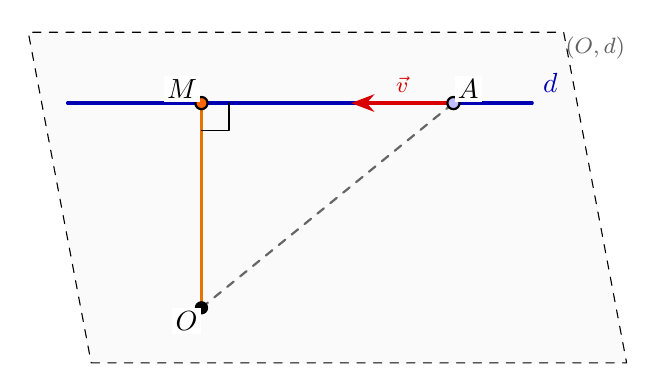
\begin{tikzpicture}[>=Stealth, line join=round, line cap=round]
    % Mặt phẳng chứa trạm radar O và quỹ đạo d
    \draw[dashed, thin, fill=gray!6, fill opacity=0.6] (-1.2,-0.9) -- (5.6,-0.9) -- (4.8,3.3) -- (-2.0,3.3) -- cycle;
    \node[right, font=\footnotesize, text=gray!75!black] at (4.7,3.1) {$(O, d)$};

    % Đường quỹ đạo bay d
    \draw[very thick, blue!70!black] (-1.5,2.4) -- (4.4,2.4) node[above right, text=blue!70!black] {$d$};

    % Các tọa độ
    \coordinate (O) at (0.2,-0.2);
    \coordinate (M) at (0.2,2.4);
    \coordinate (A) at (3.4,2.4);

    % Đoạn khoảng cách ngắn nhất OM và khoảng cách ban đầu OA
    \draw[dashed, thick, gray!80!black] (O) -- (A);
    \draw[very thick, orange!90!black] (O) -- (M);

    % Ký hiệu góc vuông tại M
    \draw[thin] (0.2,2.05) -- (0.55,2.05) -- (0.55,2.4);

    % Vectơ vận tốc v tại A hướng về phía M
    \draw[->, very thick, red!85!black] (A) -- ($(A) + (-1.3,0)$) node[midway, above, font=\footnotesize] {$\vec{v}$};

    % Điểm mốc O, M, A
    \filldraw[fill=blue!25, draw=black, thick] (A) circle (2.2pt) node[above right, fill=white, inner sep=1.2pt] {$A$};
    \filldraw[fill=orange!80!red, draw=black, thick] (M) circle (2.2pt) node[above left, fill=white, inner sep=1.2pt] {$M$};
    \filldraw[fill=black] (O) circle (2.2pt) node[below left, fill=white, inner sep=1.2pt] {$O$};
\end{tikzpicture}%
}
\end{minipage}

\item Khảo sát khối lượng của $50$ bao sản phẩm ngẫu nhiên (đơn vị: kg) được đóng gói bởi hai dây chuyền tự động I và II tại một nhà máy, người ta thu được bảng phân bố tần số ghép nhóm sau:
\begin{center}
\begin{tabular}{|c|c|c|c|c|c|}
\hline
\textbf{Khối lượng (kg)} & $[48; 49)$ & $[49; 50)$ & $[50; 51)$ & $[51; 52)$ & $[52; 53)$ \\ \hline
\textbf{Dây chuyền I} & 5 & 14 & 20 & 8 & 3 \\ \hline
\textbf{Dây chuyền II} & 3 & 20 & 22 & 4 & 1 \\ \hline
\end{tabular}
\end{center}
\begin{enumerate}[label=\textbf{\alph*)}]
    \item Khối lượng trung bình của một bao sản phẩm ở dây chuyền I là $50{,}3\text{ kg}$.
    \item Phương sai của khối lượng các bao sản phẩm ở dây chuyền I bằng $1{,}20\text{ kg}^2$.
    \item Độ lệch chuẩn của khối lượng các bao sản phẩm ở dây chuyền II bằng $0{,}80\text{ kg}$.
    \item Dây chuyền II đóng gói các bao sản phẩm có độ đồng đều cao hơn dây chuyền I.
\end{enumerate}

\end{enumerate}

% ==========================================
% PHẦN III
% ==========================================
\vspace{0.4cm}
\section*{\large PHẦN III. CÂU TRẮC NGHIỆM TRẢ LỜI NGẮN}
\textit{Thí sinh trả lời từ câu 1 đến câu 6. Mỗi câu trả lời đúng được 0,5 điểm.}

\begin{enumerate}[label=\textbf{Câu \arabic*:}, leftmargin=*]

\item Một chiếc nón lá lưu niệm có dạng hình nón tròn xoay với bán kính đáy $R = 10\text{ cm}$ và độ dài đường sinh $l = 30\text{ cm}$. Một chú kiến nhỏ xuất phát từ một điểm $A$ nằm trên đường tròn đáy bò một vòng xung quanh mặt nón rồi quay trở lại đúng điểm $A$. Quãng đường ngắn nhất mà chú kiến cần bò bằng bao nhiêu xăng-ti-mét? (kết quả làm tròn đến hàng phần mười).

\item \begin{minipage}[t]{0.55\linewidth}
Một tấm pin năng lượng mặt trời công nghệ mới có bề mặt thu sáng được giới hạn bởi hai đường cong parabol đối xứng qua trục tung $Oy$ như hình vẽ bên. Đường parabol phía trên có phương trình $y = 5 - \dfrac{1}{2}x^2$ và đường parabol phía dưới có phương trình $y = \dfrac{1}{2}x^2 - 4$ (đơn vị trên các trục là mét, với $-3 \le x \le 3$). Diện tích của bề mặt thu sáng (phần gạch chéo trong hình vẽ) bằng bao nhiêu mét vuông?
\end{minipage}\hfill
\begin{minipage}[t]{0.42\linewidth}
\vspace{-0.4\baselineskip}
\centering
\resizebox{\linewidth}{!}{%
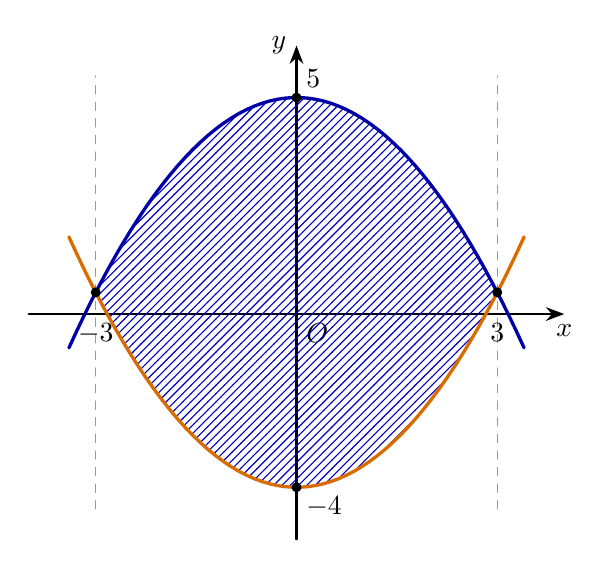
\begin{tikzpicture}[>=Stealth, x=0.85cm, y=0.55cm, line join=round, line cap=round]
    % Trục tọa độ
    \draw[->, thick] (-4.0,0) -- (4.0,0) node[below] {$x$};
    \draw[->, thick] (0,-5.2) -- (0,6.2) node[left] {$y$};
    \node[below right] at (0,0) {$O$};

    % Miền gạch chéo giữa 2 parabol từ x = -3 đến x = 3
    \fill[pattern=north east lines, pattern color=blue!75!black, domain=-3:3, samples=50] 
        plot (\x, {5 - 0.5*(\x)^2}) -- 
        plot (-\x, {0.5*(-\x)^2 - 4}) -- cycle;

    % Viền hai parabol
    \draw[very thick, blue!65!black, domain=-3.4:3.4, samples=60] plot (\x, {5 - 0.5*(\x)^2});
    \draw[very thick, orange!85!black, domain=-3.4:3.4, samples=60] plot (\x, {0.5*(\x)^2 - 4});

    % Hai biên x = -3 và x = 3
    \draw[dashed, thin, gray!80] (-3,-4.5) -- (-3,5.5);
    \draw[dashed, thin, gray!80] (3,-4.5) -- (3,5.5);

    % Tọa độ các mốc
    \node[below] at (-3,0) {$-3$};
    \node[below] at (3,0) {$3$};
    \fill (0,5) circle (1.8pt) node[above right] {$5$};
    \fill (0,-4) circle (1.8pt) node[below right] {$-4$};
    \fill (-3,0.5) circle (1.8pt);
    \fill (3,0.5) circle (1.8pt);
\end{tikzpicture}%
}
\end{minipage}

\item Một doanh nghiệp sản xuất độc quyền một loại hàng hóa. Biết hàm cầu của sản phẩm là $p(x) = 300 - 2x$ (nghìn đồng/sản phẩm), trong đó $x$ là số lượng sản phẩm sản xuất và bán ra ($x > 0$). Tổng chi phí sản xuất $x$ sản phẩm là $C(x) = x^2 + 40x + 1000$ (nghìn đồng). Ngoài ra, chính phủ áp dụng mức thuế $t = 20$ nghìn đồng trên mỗi sản phẩm bán được. Lợi nhuận lớn nhất mà doanh nghiệp có thể đạt được sau khi đã nộp thuế bằng bao nhiêu nghìn đồng?

\item Trong không gian $Oxyz$, cho mặt cầu $(S): (x - 1)^2 + (y - 2)^2 + (z - 3)^2 = 16$ và điểm $A(7; 4; 6)$. Một điểm $M$ di động trên mặt cầu $(S)$. Khoảng cách ngắn nhất giữa điểm $A$ và điểm $M$ bằng bao nhiêu?

\item \begin{minipage}[t]{0.68\linewidth}
Một cầu thủ bóng đá thực hiện 4 quả sút luân lưu $11\text{m}$. Biết rằng các lần sút là độc lập với nhau và xác suất sút thành công ở mỗi lần đều bằng $0{,}8$. Tính xác suất để cầu thủ đó sút thành công ít nhất 3 quả (kết quả làm tròn đến hàng phần trăm).
\end{minipage}\hfill
\begin{minipage}[t]{0.28\linewidth}
\vspace{-0.5\baselineskip}
\centering

\includegraphics[width=\linewidth, keepaspectratio]{cr7_penalty.jpg}
\end{minipage}

\item Cho một vật thể nằm giữa hai mặt phẳng $x = 0$ và $x = 4$. Cắt vật thể bởi mặt phẳng vuông góc với trục $Ox$ tại điểm có hoành độ $x$ ($0 \le x \le 4$), thiết diện thu được là một hình chữ nhật có hai kích thước là $\sqrt{x}$ và $6\sqrt{x}$ (đơn vị đo là mét). Thể tích của vật thể đó bằng bao nhiêu mét khối?

\end{enumerate}

% ==========================================
% BẢNG ĐÁP ÁN TỔNG HỢP (BẮT BUỘC TRANG MỚI)
% ==========================================
\newpage
\begin{center}
    {\Large\textbf{BẢNG ĐÁP ÁN TỔNG HỢP}}\\[4pt]
    \textbf{ĐỀ SỐ 10 - MÔN: TOÁN}
\end{center}
\vspace{0.3cm}

\noindent\textbf{\large PHẦN I. CÂU TRẮC NGHIỆM NHIỀU PHƯƠNG ÁN LỰA CHỌN}
\begin{center}
\renewcommand{\arraystretch}{1.25}
\begin{tabular}{|c|c|c|c|c|c|c|c|c|c|c|c|}
\hline
\textbf{1} & \textbf{2} & \textbf{3} & \textbf{4} & \textbf{5} & \textbf{6} & \textbf{7} & \textbf{8} & \textbf{9} & \textbf{10} & \textbf{11} & \textbf{12} \\ \hline
\textbf{B} & \textbf{D} & \textbf{A} & \textbf{C} & \textbf{B} & \textbf{D} & \textbf{A} & \textbf{C} & \textbf{B} & \textbf{D} & \textbf{A} & \textbf{C} \\ \hline
\end{tabular}
\end{center}

\vspace{0.3cm}
\noindent\textbf{\large PHẦN II. CÂU TRẮC NGHIỆM ĐÚNG SAI}
\begin{center}
\renewcommand{\arraystretch}{1.25}
\begin{tabular}{|c|c|c|c|c|}
\hline
\textbf{Câu} & \textbf{Ý a)} & \textbf{Ý b)} & \textbf{Ý c)} & \textbf{Ý d)} \\ \hline
\textbf{Câu 1} & Đ & Đ & S & Đ \\ \hline
\textbf{Câu 2} & Đ & S & Đ & Đ \\ \hline
\textbf{Câu 3} & Đ & Đ & S & Đ \\ \hline
\textbf{Câu 4} & Đ & S & Đ & Đ \\ \hline
\end{tabular}
\end{center}

\vspace{0.3cm}
\noindent\textbf{\large PHẦN III. CÂU TRẮC NGHIỆM TRẢ LỜI NGẮN}
\begin{center}
\renewcommand{\arraystretch}{1.25}
\begin{tabular}{|c|c|c|c|c|c|}
\hline
\textbf{Câu 1} & \textbf{Câu 2} & \textbf{Câu 3} & \textbf{Câu 4} & \textbf{Câu 5} & \textbf{Câu 6} \\ \hline
52,0 & 36 & 3800 & 3 & 0,82 & 48 \\ \hline
\end{tabular}
\end{center}

% ==========================================
% HƯỚNG DẪN GIẢI CHI TIẾT
% ==========================================
\newpage
\begin{center}
    {\Large\textbf{HƯỚNG DẪN GIẢI CHI TIẾT}}\\[4pt]
    \textbf{ĐỀ SỐ 10 - MÔN: TOÁN}
\end{center}
\vspace{0.3cm}

\section*{\large PHẦN I. CÂU TRẮC NGHIỆM NHIỀU PHƯƠNG ÁN LỰA CHỌN}

\noindent\textbf{Câu 1.} Ta thực hiện phép chia đa thức tử cho mẫu:
\[
\dfrac{2x^2 + x - 3}{x + 1} = 2x - 1 - \dfrac{2}{x + 1}.
\]
Vì $\lim\limits_{x \to \pm\infty} \left[ y - (2x - 1) \right] = \lim\limits_{x \to \pm\infty} \left( -\dfrac{2}{x + 1} \right) = 0$ nên đường thẳng $y = 2x - 1$ là đường tiệm cận xiên của đồ thị $(C)$.\\
\textbf{Chọn B.}

\vspace{0.25cm}
\noindent\textbf{Câu 2.} Hàm số xác định khi và chỉ khi:
\[
\begin{cases}
9 - x^2 > 0 \\
x - 1 \ne 0
\end{cases}
\iff
\begin{cases}
-3 < x < 3 \\
x \ne 1
\end{cases}
\iff x \in (-3; 3) \setminus \{1\}.
\]
Vậy tập xác định của hàm số là $D = (-3; 3) \setminus \{1\}$.\\
\textbf{Chọn D.}

\vspace{0.25cm}
\noindent\textbf{Câu 3.} Với $x \in \left(-\dfrac{3}{2}; +\infty\right)$, ta có $2x + 3 > 0$, do đó:
\[
\int \dfrac{1}{2x + 3}\,\text{d}x = \dfrac{1}{2}\ln|2x + 3| + C = \dfrac{1}{2}\ln(2x + 3) + C.
\]
\textbf{Chọn A.}

\vspace{0.25cm}
\noindent\textbf{Câu 4.} Đường thẳng $d$ có một vectơ chỉ phương là $\vec{u}_d = (2; -3; 5)$.\\
Mọi vectơ cùng phương với $\vec{u}_d$ đều là vectơ chỉ phương của $d$.\\
Xét vectơ $\vec{u}_3 = (-4; 6; -10) = -2\vec{u}_d$, do đó $\vec{u}_3$ là một vectơ chỉ phương của đường thẳng $d$.\\
\textbf{Chọn C.}

\vspace{0.25cm}
\noindent\textbf{Câu 5.} Gọi $A$ là biến cố "Cảm biến thứ nhất kích hoạt báo động", $B$ là biến cố "Cảm biến thứ hai kích hoạt báo động".\\
Theo đề bài, $A$ và $B$ độc lập, với $P(A) = 0{,}8$ và $P(B) = 0{,}7$.\\
Xác suất để cả hai cảm biến cùng không kích hoạt là:
\[
P(\overline{A} \cap \overline{B}) = P(\overline{A}) \cdot P(\overline{B}) = (1 - 0{,}8)(1 - 0{,}7) = 0{,}2 \times 0{,}3 = 0{,}06.
\]
Xác suất để có ít nhất một cảm biến kích hoạt thành công là:
\[
P = 1 - P(\overline{A} \cap \overline{B}) = 1 - 0{,}06 = 0{,}94.
\]
\textbf{Chọn B.}

\vspace{0.25cm}
\noindent\textbf{Câu 6.} Cỡ mẫu là $n = 4 + 8 + 14 + 10 + 4 = 40$.\\
Tứ phân vị thứ nhất $Q_1$ ứng với giá trị $\dfrac{n}{4} = \dfrac{40}{4} = 10$.\\
Tần số tích lũy của nhóm $[4; 5)$ là $cf_1 = 4 < 10$.\\
Tần số tích lũy của nhóm $[5; 6)$ là $cf_2 = 4 + 8 = 12 \ge 10$.\\
Do đó, nhóm chứa tứ phân vị thứ nhất là $[5; 6)$, với đầu mút trái $L = 5$, độ dài nhóm $h = 6 - 5 = 1$, tần số nhóm $f_2 = 8$, và tần số tích lũy nhóm đứng trước $cf_1 = 4$.\\
Áp dụng công thức:
\[
Q_1 = 5 + \dfrac{10 - 4}{8} \cdot 1 = 5 + \dfrac{6}{8} = 5 + 0{,}75 = 5{,}75.
\]
\textbf{Chọn D.}

\vspace{0.25cm}
\noindent\textbf{Câu 7.} Ta có $SA \perp (ABC) \implies SA \perp BC$.\\
Mặt khác, tam giác $ABC$ vuông tại $B$ nên $AB \perp BC$.\\
Từ đó suy ra $BC \perp (SAB)$, dẫn đến $BC \perp SB$.\\
Vì $SB \perp BC$ (trong $(SBC)$) và $AB \perp BC$ (trong $(ABC)$) nên góc phẳng nhị diện $[S, BC, A]$ chính là góc $\widehat{SBA}$.\\
Trong tam giác vuông $SAB$ tại $A$, ta có $SA = AB = a$, do đó tam giác $SAB$ vuông cân tại $A$, suy ra $\widehat{SBA} = 45^\circ$.\\
\textbf{Chọn A.}

\vspace{0.25cm}
\noindent\textbf{Câu 8.} Số hạng tổng quát của cấp số nhân là $u_n = u_1 \cdot q^{n-1}$.\\
Với $n = 4$, ta có:
\[
u_4 = u_1 \cdot q^3 = 2 \cdot (-3)^3 = 2 \cdot (-27) = -54.
\]
\textbf{Chọn C.}

\vspace{0.25cm}
\noindent\textbf{Câu 9.} Độ pH ban đầu của dung dịch là:
\[
\text{pH}_1 = -\log_{10}(10^{-5}) = 5.
\]
Sau khi pha thêm nước, độ pH mới của dung dịch là:
\[
\text{pH}_2 = -\log_{10}(10^{-7}) = 7.
\]
Độ biến thiên pH là: $\Delta\text{pH} = \text{pH}_2 - \text{pH}_1 = 7 - 5 = 2$, tức là độ pH đã tăng thêm 2 đơn vị.\\
\textbf{Chọn B.}

\vspace{0.25cm}
\noindent\textbf{Câu 10.} Phương trình mặt cầu $(S): x^2 + y^2 + z^2 - 4x + 2y - 6z + 5 = 0$ có các hệ số:
\[
a = 2,\quad b = -1,\quad c = 3,\quad d = 5.
\]
Tâm mặt cầu là $I(2; -1; 3)$.\\
Bán kính mặt cầu là:
\[
R = \sqrt{a^2 + b^2 + c^2 - d} = \sqrt{2^2 + (-1)^2 + 3^2 - 5} = \sqrt{4 + 1 + 9 - 5} = \sqrt{9} = 3.
\]
\textbf{Chọn D.}

\vspace{0.25cm}
\noindent\textbf{Câu 11.} Hàm lợi nhuận thu được là:
\[
L(x) = R(x) - C(x) = (120x - x^2) - (20x + 100) = -x^2 + 100x - 100.
\]
Đạo hàm: $L'(x) = -2x + 100$. Cho $L'(x) = 0 \iff x = 50$.\\
Vì hệ số $a = -1 < 0$ nên hàm số $L(x)$ đạt giá trị lớn nhất tại đỉnh parabol $x = 50 \in [0; 100]$.\\
Vậy xưởng cần sản xuất $50$ sản phẩm.\\
\textbf{Chọn A.}

\vspace{0.25cm}
\noindent\textbf{Câu 12.} Diện tích đáy tam giác vuông $ABC$ là:
\[
S_{ABC} = \dfrac{1}{2} AB \cdot AC = \dfrac{1}{2} \cdot 3a \cdot 4a = 6a^2.
\]
Thể tích khối lăng trụ đứng là $V = S_{ABC} \cdot AA'$, suy ra:
\[
AA' = \dfrac{V}{S_{ABC}} = \dfrac{36a^3}{6a^2} = 6a.
\]
\textbf{Chọn C.}

% ==========================================
\vspace{0.4cm}
\section*{\large PHẦN II. CÂU TRẮC NGHIỆM ĐÚNG SAI}

\noindent\textbf{Câu 1.}
Tập xác định: $D = \mathbb{R} \setminus \{1\}$. Ta có $y = \dfrac{x^2 - x + 1}{x - 1} = x + \dfrac{1}{x - 1}$.\\
Đạo hàm:
\[
y' = 1 - \dfrac{1}{(x - 1)^2} = \dfrac{(x - 1)^2 - 1}{(x - 1)^2} = \dfrac{x^2 - 2x}{(x - 1)^2}.
\]
Cho $y' = 0 \iff x = 0$ hoặc $x = 2$.\\
Bảng biến thiên:
\begin{itemize}
    \item Trên $(-\infty; 0)$ và $(2; +\infty)$: $y' > 0$, hàm số đồng biến.
    \item Trên $(0; 1)$ và $(1; 2)$: $y' < 0$, hàm số nghịch biến.
\end{itemize}
Do đó, hàm số đạt cực đại tại $x = 0$ với $y(0) = -1$; đạt cực tiểu tại $x = 2$ với $y(2) = 3$.\\
$\implies$ \textbf{a) ĐÚNG.}

Đường thẳng đi qua hai điểm cực trị của hàm phân thức bậc hai trên bậc nhất $y = \dfrac{u(x)}{v(x)}$ có phương trình là $y = \dfrac{u'(x)}{v'(x)} = \dfrac{2x - 1}{1} = 2x - 1$.\\
Kiểm tra: với cực đại $(0; -1) \implies -1 = 2(0) - 1$; với cực tiểu $(2; 3) \implies 3 = 2(2) - 1$ (thỏa mãn).\\
$\implies$ \textbf{b) ĐÚNG.}

Đường tiệm cận đứng là $x = 1$. Đường tiệm cận xiên là $y = x$.\\
Giao điểm của hai đường tiệm cận là nghiệm của hệ $\begin{cases} x = 1 \\ y = x \end{cases} \implies I(1; 1)$, không phải $(1; 2)$.\\
$\implies$ \textbf{c) SAI.}

Tại điểm có hoành độ $x = 2$, ta có hệ số góc tiếp tuyến là $k = y'(2) = 0$.\\
Tọa độ tiếp điểm là $(2; 3)$. Phương trình tiếp tuyến là $y - 3 = 0(x - 2) \iff y = 3$.\\
Đường thẳng này song song với trục hoành $Ox$.\\
$\implies$ \textbf{d) ĐÚNG.}

\vspace{0.3cm}
\noindent\textbf{Câu 2.}
Gọi $B$ là biến cố "Người được chọn mắc bệnh", $T$ là biến cố "Người được chọn có kết quả xét nghiệm dương tính".\\
Theo đề bài:
\[
P(B) = 0{,}01 \implies P(\overline{B}) = 0{,}99.
\]
\[
P(T|B) = 0{,}98 \implies P(\overline{T}|B) = 0{,}02.
\]
\[
P(\overline{T}|\overline{B}) = 0{,}95 \implies P(T|\overline{B}) = 0{,}05.
\]
Theo công thức xác suất toàn phần:
\[
P(T) = P(B) \cdot P(T|B) + P(\overline{B}) \cdot P(T|\overline{B}) = 0{,}01 \cdot 0{,}98 + 0{,}99 \cdot 0{,}05 = 0{,}0098 + 0{,}0495 = 0{,}0593.
\]
$\implies$ \textbf{a) ĐÚNG.}

Theo công thức Bayes, xác suất một người thực sự mắc bệnh khi đã nhận kết quả dương tính là:
\[
P(B|T) = \dfrac{P(B \cap T)}{P(T)} = \dfrac{0{,}0098}{0{,}0593} \approx 0{,}1653 = 16{,}53\% < 50\%.
\]
$\implies$ \textbf{b) SAI.}

Xác suất một người vừa không mắc bệnh vừa có kết quả xét nghiệm âm tính là:
\[
P(\overline{B} \cap \overline{T}) = P(\overline{B}) \cdot P(\overline{T}|\overline{B}) = 0{,}99 \cdot 0{,}95 = 0{,}9405.
\]
$\implies$ \textbf{c) ĐÚNG.}

Xác suất một người nhận kết quả âm tính là:
\[
P(\overline{T}) = 1 - P(T) = 1 - 0{,}0593 = 0{,}9407.
\]
Xác suất người đó vẫn mắc bệnh khi kết quả âm tính là:
\[
P(B|\overline{T}) = \dfrac{P(B \cap \overline{T})}{P(\overline{T})} = \dfrac{P(B) \cdot P(\overline{T}|B)}{P(\overline{T})} = \dfrac{0{,}01 \cdot 0{,}02}{0{,}9407} = \dfrac{0{,}0002}{0{,}9407} \approx 0{,}000213 = 0{,}0213\% < 0{,}05\%.
\]
$\implies$ \textbf{d) ĐÚNG.}

\vspace{0.3cm}
\noindent\textbf{Câu 3.}
Vị trí ban đầu của drone là $A(8; 6; 4)$. Khoảng cách từ trạm radar $O(0; 0; 0)$ đến $A$ là:
\[
OA = \sqrt{8^2 + 6^2 + 4^2} = \sqrt{64 + 36 + 16} = \sqrt{116} = 2\sqrt{29}\text{ km}.
\]
$\implies$ \textbf{a) ĐÚNG.}

Vị trí của drone tại thời điểm $t$ là $M(8 - 2t; 6 - t; 4 + t)$.\\
Xét điểm $B(2; 3; 7)$, giải hệ phương trình:
\[
\begin{cases}
8 - 2t = 2 \\
6 - t = 3 \\
4 + t = 7
\end{cases}
\iff t = 3.
\]
Hệ có nghiệm duy nhất $t = 3 \ge 0$, do đó quỹ đạo bay của drone đi qua điểm $B(2; 3; 7)$.\\
$\implies$ \textbf{b) ĐÚNG.}

Bình phương khoảng cách từ $O$ đến $M$ tại thời điểm $t$ là:
\begin{align*}
d^2(t) = OM^2 &= (8 - 2t)^2 + (6 - t)^2 + (4 + t)^2 \\
&= (4t^2 - 32t + 64) + (t^2 - 12t + 36) + (t^2 + 8t + 16) = 6t^2 - 36t + 116.
\end{align*}
Tam thức bậc hai $f(t) = 6t^2 - 36t + 116$ có hệ số $a = 6 > 0$ nên đạt giá trị nhỏ nhất tại đỉnh:
\[
t = -\dfrac{b}{2a} = -\dfrac{-36}{2 \cdot 6} = 3\text{ giờ} \ne 2\text{ giờ}.
\]
$\implies$ \textbf{c) SAI.}

Tại $t = 3$, khoảng cách ngắn nhất là:
\[
OM_{\min} = \sqrt{f(3)} = \sqrt{6(3)^2 - 36(3) + 116} = \sqrt{54 - 108 + 116} = \sqrt{62}\text{ km}.
\]
$\implies$ \textbf{d) ĐÚNG.}

\vspace{0.3cm}
\noindent\textbf{Câu 4.}
Giá trị đại diện của các nhóm lần lượt là:
\[
x_1 = 48{,}5;\quad x_2 = 49{,}5;\quad x_3 = 50{,}5;\quad x_4 = 51{,}5;\quad x_5 = 52{,}5.
\]
\textbf{Xét dây chuyền I ($n = 50$):}
Khối lượng trung bình:
\begin{align*}
\overline{x}_1 &= \dfrac{5 \cdot 48{,}5 + 14 \cdot 49{,}5 + 20 \cdot 50{,}5 + 8 \cdot 51{,}5 + 3 \cdot 52{,}5}{50} \\
&= \dfrac{242{,}5 + 693 + 1010 + 412 + 157{,}5}{50} = \dfrac{2515}{50} = 50{,}3\text{ kg}.
\end{align*}
$\implies$ \textbf{a) ĐÚNG.}

Phương sai của dây chuyền I:
\begin{align*}
s_1^2 &= \dfrac{1}{50} \left[ 5(48{,}5 - 50{,}3)^2 + 14(49{,}5 - 50{,}3)^2 + 20(50{,}5 - 50{,}3)^2 + 8(51{,}5 - 50{,}3)^2 + 3(52{,}5 - 50{,}3)^2 \right] \\
&= \dfrac{1}{50} \left[ 5(-1{,}8)^2 + 14(-0{,}8)^2 + 20(0{,}2)^2 + 8(1{,}2)^2 + 3(2{,}2)^2 \right] \\
&= \dfrac{1}{50} \left[ 5 \cdot 3{,}24 + 14 \cdot 0{,}64 + 20 \cdot 0{,}04 + 8 \cdot 1{,}44 + 3 \cdot 4{,}84 \right] \\
&= \dfrac{1}{50} \left[ 16{,}2 + 8{,}96 + 0{,}8 + 11{,}52 + 14{,}52 \right] = \dfrac{52{,}0}{50} = 1{,}04\text{ kg}^2 \ne 1{,}20\text{ kg}^2.
\end{align*}
$\implies$ \textbf{b) SAI.}

\textbf{Xét dây chuyền II ($n = 50$):}
Khối lượng trung bình:
\begin{align*}
\overline{x}_2 &= \dfrac{3 \cdot 48{,}5 + 20 \cdot 49{,}5 + 22 \cdot 50{,}5 + 4 \cdot 51{,}5 + 1 \cdot 52{,}5}{50} \\
&= \dfrac{145{,}5 + 990 + 1111 + 206 + 52{,}5}{50} = \dfrac{2505}{50} = 50{,}1\text{ kg}.
\end{align*}
Phương sai của dây chuyền II:
\begin{align*}
s_2^2 &= \dfrac{1}{50} \left[ 3(48{,}5 - 50{,}1)^2 + 20(49{,}5 - 50{,}1)^2 + 22(50{,}5 - 50{,}1)^2 + 4(51{,}5 - 50{,}1)^2 + 1(52{,}5 - 50{,}1)^2 \right] \\
&= \dfrac{1}{50} \left[ 3(-1{,}6)^2 + 20(-0{,}6)^2 + 22(0{,}4)^2 + 4(1{,}4)^2 + 1(2{,}4)^2 \right] \\
&= \dfrac{1}{50} \left[ 3 \cdot 2{,}56 + 20 \cdot 0{,}36 + 22 \cdot 0{,}16 + 4 \cdot 1{,}96 + 1 \cdot 5{,}76 \right] \\
&= \dfrac{1}{50} \left[ 7{,}68 + 7{,}20 + 3{,}52 + 7{,}84 + 5{,}76 \right] = \dfrac{32{,}0}{50} = 0{,}64\text{ kg}^2.
\end{align*}
Độ lệch chuẩn của dây chuyền II: $s_2 = \sqrt{0{,}64} = 0{,}80\text{ kg}$.\\
$\implies$ \textbf{c) ĐÚNG.}

Vì $s_2 = 0{,}80\text{ kg} < s_1 = \sqrt{1{,}04} \approx 1{,}02\text{ kg}$ nên độ phân tán khối lượng của dây chuyền II nhỏ hơn dây chuyền I, nghĩa là dây chuyền II đóng gói đồng đều hơn.\\
$\implies$ \textbf{d) ĐÚNG.}

% ==========================================
\vspace{0.4cm}
\section*{\large PHẦN III. CÂU TRẮC NGHIỆM TRẢ LỜI NGẮN}

\noindent\textbf{Câu 1.} Khi cắt mặt xung quanh của hình nón dọc theo một đường sinh và trải phẳng ra một mặt phẳng, ta nhận được một hình quạt tròn tâm $S$, bán kính bằng độ dài đường sinh $l = 30\text{ cm}$.\\
Độ dài cung tròn của hình quạt bằng chu vi đáy hình nón: $C = 2\pi R = 2\pi \cdot 10 = 20\pi\text{ cm}$.\\
Góc ở đỉnh hình quạt tròn là:
\[
\alpha = \dfrac{2\pi R}{l} = \dfrac{20\pi}{30} = \dfrac{2\pi}{3} = 120^\circ.
\]
Chú kiến xuất phát từ điểm $A$ trên vành đáy, bò một vòng xung quanh nón rồi trở về điểm $A$. Trên mặt phẳng trải rộng, điểm xuất phát là $A$ và điểm đích là $A'$ trên hai cạnh biên $SA$ và $SA'$ của hình quạt tròn ($SA = SA' = 30\text{ cm}$, $\widehat{ASA'} = 120^\circ$).\\
Quãng đường ngắn nhất chính là độ dài đoạn thẳng $AA'$. Áp dụng định lí cosin trong tam giác cân $SAA'$:
\[
AA' = \sqrt{SA^2 + SA'^2 - 2 \cdot SA \cdot SA' \cdot \cos 120^\circ} = \sqrt{30^2 + 30^2 - 2 \cdot 30^2 \cdot \left(-\dfrac{1}{2}\right)} = 30\sqrt{3}\text{ cm}.
\]
Tính toán xấp xỉ: $AA' = 30\sqrt{3} \approx 51{,}9615\text{ cm}$. Làm tròn đến hàng phần mười ta được $52{,}0$.\\
\textbf{Đáp số: 52,0.}

\vspace{0.3cm}
\noindent\textbf{Câu 2.} Trên đoạn $[-3; 3]$, xét hiệu giữa hai hàm số:
\[
y_1 - y_2 = \left(5 - \dfrac{1}{2}x^2\right) - \left(\dfrac{1}{2}x^2 - 4\right) = 9 - x^2.
\]
Với mọi $x \in [-3; 3]$, ta có $9 - x^2 \ge 0 \implies y_1 \ge y_2$. Do đó đồ thị parabol bề lõm quay xuống nằm phía trên parabol bề lõm quay lên.\\
Diện tích của bề mặt thu sáng (phần gạch chéo) được tính bằng tích phân:
\[
S = \int_{-3}^3 (y_1 - y_2)\,\text{d}x = \int_{-3}^3 (9 - x^2)\,\text{d}x = 2\int_0^3 (9 - x^2)\,\text{d}x = 2 \left[ 9x - \dfrac{x^3}{3} \right]_0^3 = 2 \left( 27 - 9 \right) = 36\text{ m}^2.
\]
\textbf{Đáp số: 36.}

\vspace{0.3cm}
\noindent\textbf{Câu 3.} Doanh thu khi bán $x$ sản phẩm là:
\[
R(x) = x \cdot p(x) = x(300 - 2x) = 300x - 2x^2\text{ (nghìn đồng)}.
\]
Tổng chi phí nộp thuế khi sản xuất và bán $x$ sản phẩm là:
\[
T(x) = t \cdot x = 20x\text{ (nghìn đồng)}.
\]
Lợi nhuận của doanh nghiệp sau khi nộp thuế là:
\[
L(x) = R(x) - C(x) - T(x) = (300x - 2x^2) - (x^2 + 40x + 1000) - 20x = -3x^2 + 240x - 1000\text{ (nghìn đồng)}.
\]
Đạo hàm: $L'(x) = -6x + 240$. Cho $L'(x) = 0 \iff x = 40$ (sản phẩm).\\
Hàm $L(x)$ là tam thức bậc hai có hệ số $a = -3 < 0$ nên đạt giá trị lớn nhất tại $x = 40$:
\[
L_{\max} = L(40) = -3(40)^2 + 240(40) - 1000 = -4800 + 9600 - 1000 = 3800\text{ (nghìn đồng)}.
\]
\textbf{Đáp số: 3800.}

\vspace{0.3cm}
\noindent\textbf{Câu 4.} Mặt cầu $(S)$ có tâm $I(1; 2; 3)$ và bán kính $R = \sqrt{16} = 4$.\\
Khoảng cách từ tâm $I$ đến điểm $A(7; 4; 6)$ là:
\[
IA = \sqrt{(7 - 1)^2 + (4 - 2)^2 + (6 - 3)^2} = \sqrt{6^2 + 2^2 + 3^2} = \sqrt{36 + 4 + 9} = \sqrt{49} = 7.
\]
Vì $IA = 7 > R = 4$ nên điểm $A$ nằm ngoài mặt cầu $(S)$.\\
Khi điểm $M$ di động trên mặt cầu $(S)$, khoảng cách ngắn nhất giữa $A$ và $M$ đạt được khi $M$ là giao điểm của đoạn thẳng $IA$ với mặt cầu $(S)$:
\[
AM_{\min} = IA - R = 7 - 4 = 3.
\]
\textbf{Đáp số: 3.}

\vspace{0.3cm}
\noindent\textbf{Câu 5.} Gọi $X$ là số lần sút thành công trong 4 lần sút độc lập. Biến ngẫu nhiên $X$ tuân theo phân bố nhị thức với $n = 4$ và xác suất thành công ở mỗi lần là $p = 0{,}8$ (xác suất thất bại $q = 1 - p = 0{,}2$).\\
Biến cố "Sút thành công ít nhất 3 quả" tương ứng với $X \ge 3$, tức là $X = 3$ hoặc $X = 4$.\\
Xác suất để sút thành công đúng 3 quả là:
\[
P(X = 3) = C_4^3 \cdot (0{,}8)^3 \cdot (0{,}2)^1 = 4 \cdot 0{,}512 \cdot 0{,}2 = 0{,}4096.
\]
Xác suất để sút thành công cả 4 quả là:
\[
P(X = 4) = C_4^4 \cdot (0{,}8)^4 \cdot (0{,}2)^0 = 1 \cdot 0{,}4096 \cdot 1 = 0{,}4096.
\]
Xác suất để sút thành công ít nhất 3 quả là:
\[
P(X \ge 3) = P(X = 3) + P(X = 4) = 0{,}4096 + 0{,}4096 = 0{,}8192.
\]
Làm tròn kết quả đến hàng phần trăm ta được $0{,}82$.\\
\textbf{Đáp số: 0,82.}

\vspace{0.3cm}
\noindent\textbf{Câu 6.} Theo giả thiết, thiết diện của vật thể khi cắt bởi mặt phẳng vuông góc với trục $Ox$ tại hoành độ $x \in [0; 4]$ là hình chữ nhật có kích thước $\sqrt{x}$ và $6\sqrt{x}$.\\
Diện tích của thiết diện đó là:
\[
S(x) = \sqrt{x} \cdot 6\sqrt{x} = 6x\text{ (với mọi } 0 \le x \le 4\text{)}.
\]
Thể tích của vật thể được giới hạn bởi hai mặt phẳng $x = 0$ và $x = 4$ là:
\[
V = \int_0^4 S(x)\,\text{d}x = \int_0^4 6x\,\text{d}x = \left[ 3x^2 \right]_0^4 = 3 \cdot 4^2 - 0 = 3 \cdot 16 = 48\text{ m}^3.
\]
\textbf{Đáp số: 48.}

\end{document}
